\section{Challenges for imaging MeerKAT data} \label{meerkat}
New interferometers like MeerKAT put additional challenges on the image reconstruction problem. First, the new instrument produce a new magnitude of data, forcing reconstruction algorithms to be highly scalable and distributable. Second, the more sensitive instruments with large field of view amplify effects which were negligible in older instruments, like non-coplanar baselines or the ionosphere.

Compressed sensing has to be able to work with these issues somehow. Solutions all in the context of the major cycle, a new architecture may need to handle effects differently. Hopefully in a manner that is at least as efficient.

In this work, the effects of non-coplanar baselines gets handled in more detail. The effect has a neat mathematical notation, it adds a third fourier component to the measurement equation, but breaks the two dimensional fourier relationship introduced in section \ref{intro:basic}. 

Calibration used to be a task before image reconstruction.
Calibration gets not explicitly handled here, but it is important to keep in mind. For older interferometers, the data was calibrated before image reconstruction. With the advent of self-calibration, the image reconstruction is also used to improve calibration. MeerKAT requires more calibration parameters, so an image reconstruction algorithm has to be able to calibrate, or it is not interesting.



Further issues that do not get handled here
\begin{itemize}
	\item (Beam Pattern, A Projection)
	\item Full polarization
	\item Wide band imaging
\end{itemize}

There are several challenger for imaging meerkat data. One problem is the new amount of data.

terabytes of measurements. Large image size 32k squared are the obvious problems to solve. Distributing the problem is not part of this work.

 In this work, it is focused on Wide field of view issue. 







\subsection{Wide Field of View Imaging and the third Fourier Component} \label{meerkat:wof}
The measurement equation of radio interferometers contains a third fourier component, the $w$ component. This leads to the following measurement equation \eqref{meerkat:ftsphere}.

\begin{equation}\label{meerkat:ftsphere}
V(u, v, w) = \int\int \frac{I(x, y)}{\sqrt{1 - x^2 - y ^2}} e^{2 \pi i [ux+vy+ w(\sqrt{1 - x^2 - y ^2} - 1)]} \: dx \: dy
\end{equation}

For small field of view observations, the term $\sqrt{1 - x^2 - y ^2} \approx 1$, and we arrive at the basic measurement equation \eqref{intro:basic}. For small field of view, the $w$ term can be ignored, and the image can be calculated with the inverse two dimensional non-uniform FFT. For wide field of view measurements, the $w$ term breaks the two dimensional Fourier relationship. The measurement equation \eqref{meerkat:ftsphere} can still be inverted, but the resulting algorithm has a quadratic runtime and is not feasible in practice.

Note that the image $I(x,y)$ of the wide field of view the measurement equation \eqref{meerkat:ftsphere} is still two dimensional, even though the Visibilities $V(u, v, w)$ have three. The relationship between Visibilities and image is neither the two, nor the three dimensional Fourier transform. The Visibilities represents an image on the celestial sphere. This means the image is naturally curved, and the $w$ component represents the distortion introduced by the curvature.

One can simply ignore the $w$ component, ignore the curvature and use the two dimensional Fourier Transform. The image then does not lie on a sphere, but on a tangent plane. At the tangent point (where $\sqrt{1 - x^2 - y ^2} \approx 1$, typically the image center in radio astronomy) the two reconstructions are identical. But the distortion gets more severe away from the tangent point. The image \ref{meerkat:2dfft} shows a tangent plane reconstruction over a large field of view, while \ref{meerkat:wcorrection} shows the same reconstruction but $w$ corrected. Close to the tangent point, the image center, the reconstructions both locate the point sources. At the image edges, the distortion gets severe enough to decorrelate the Visibilities and the point sources get 'torn' apart.

\begin{figure}[h]
	\centering
	\begin{subfigure}[b]{0.45\linewidth}
		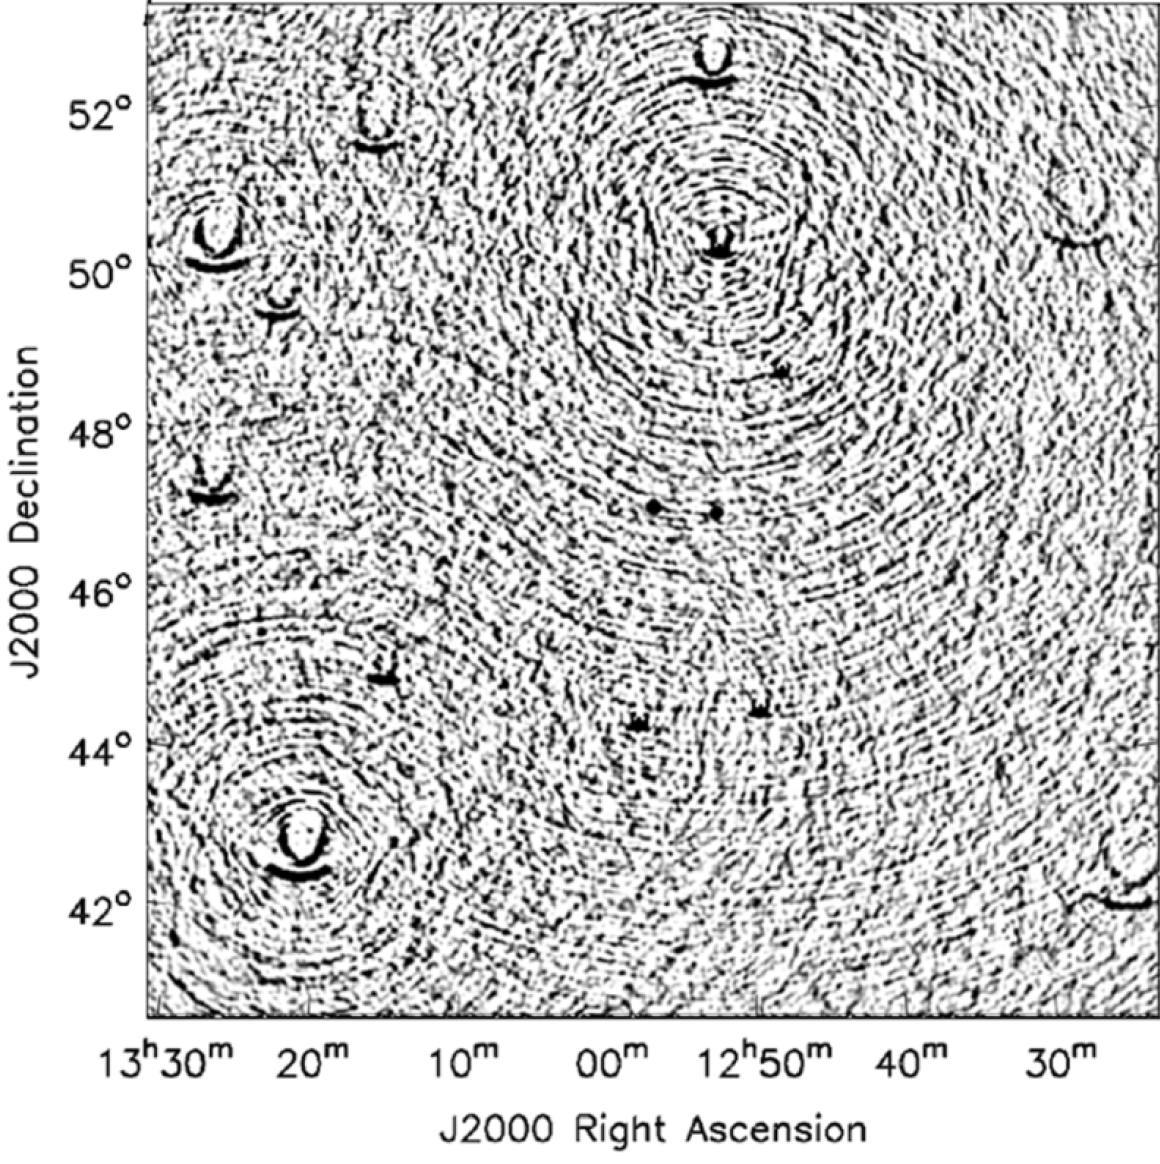
\includegraphics[width=\linewidth]{./chapters/03.challenges/w-no-correction.png}
		\caption{2D Fourier Transform.}
		\label{meerkat:2dfft}
	\end{subfigure}
	\begin{subfigure}[b]{0.45\linewidth}
		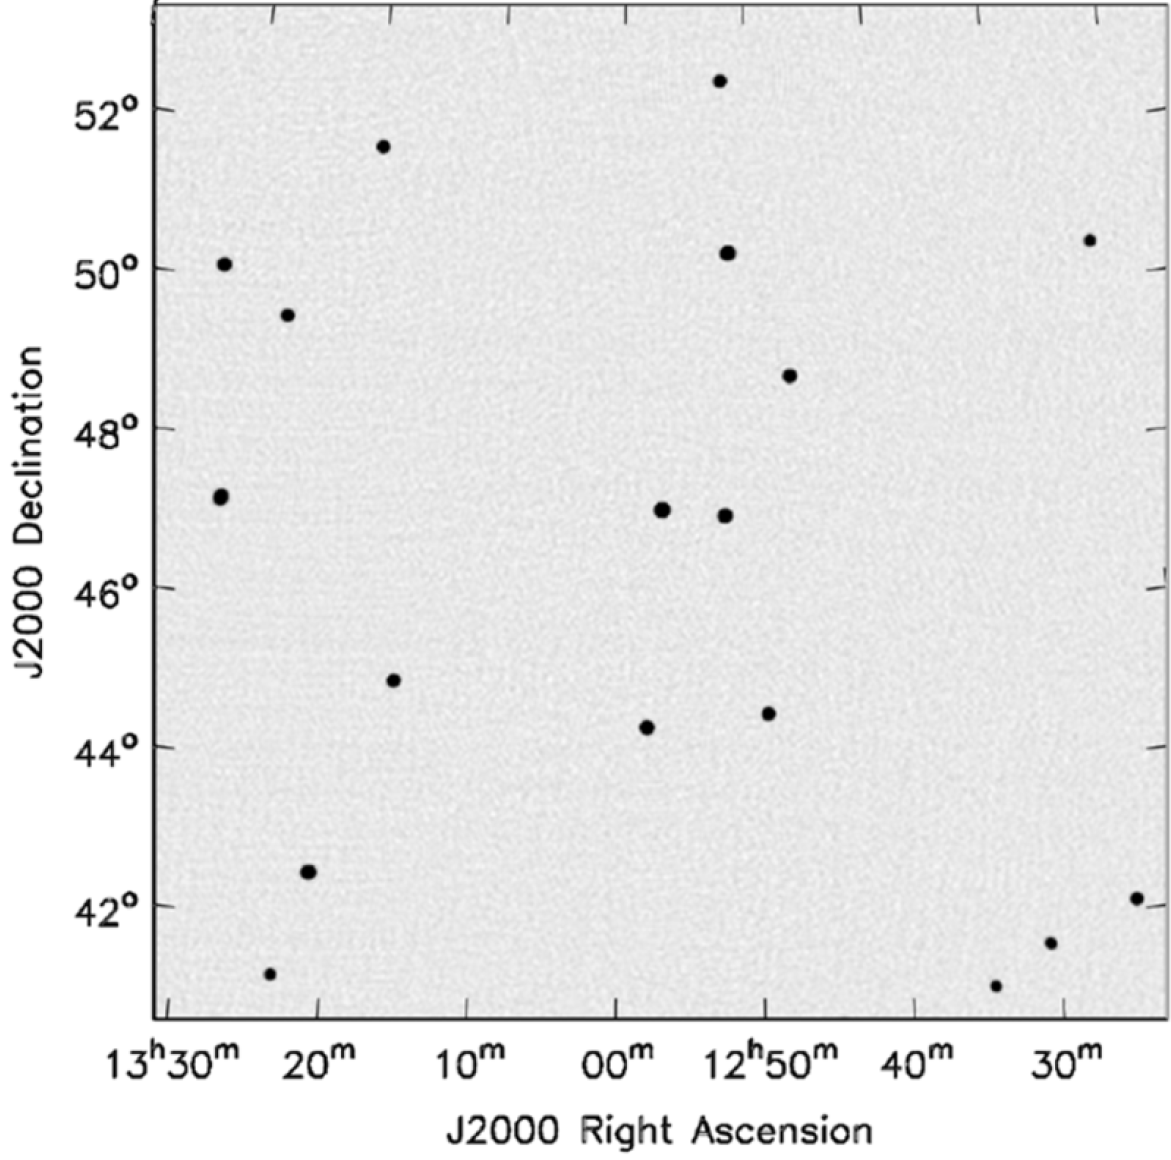
\includegraphics[width=\linewidth]{./chapters/03.challenges/w-correction.png}
		\caption{Fourier Transform with $w$-correction.}
		\label{meerkat:wcorrection}
	\end{subfigure}
	\caption{Celestial sphere distortion on simulated data. Source: \cite{cornwell2008noncoplanar}}
	\label{meerkat:wdistortion}
\end{figure}

Image reconstructions for MeerKAT need to account for the $w$ component efficiently. In the Major Cycle framework, this is part of the non-uniform FFT. The first approach was to image facets, creating several tangent planes for the celestial sphere. A more efficient approach came in the form of the $w$-projection algorithm\cite{cornwell2008noncoplanar}. It uses convolution on the Visibilities during the non-uniform FFT. MeerKAT currently uses the $w$-stacking algorithm, which more efficient than $w$-projection on MeerKAT's data volume and is simple to distribute.


This is still an active field of research. The latest work as of time of writing is a hybrid approach\cite{pratley2018fast} with both $w$-stacking and $w$-projection. As of time of writing, it was not yet adapted.


\subsubsection{State of the art: $w$-stacking algorithm}
Here a short explanation of the w-stacking algorithm is provided. It is a surprisingly simple algorithm that seems to be here to stay. It is a modification of the nuFFT operation displayed in figure \ref{intro:major}. 


\textit{Inverse nuFFT with w-stacking}:
Visibilities get grouped into stacks by their $w$-term. Every visibility inside a stack has a similar $w$-term. The more stacks, the more accurately you can handle the $w$ component. The figure displays the relation

The nuFFT gets called on each stack separately, and a constant $w$ correction factor applied. Since $w$-term is constant, we can use the two dimensional nuFFT again. At the end, all the stacks are summed together to form the dirty image. 

\textit{nuFFT with w-stacking}:
The inverse is done in a similar fashion. The sum cannot be re-separated, so the image gets copied into each stack. The constant $w$ factor gets divided out. The nuFFT gets applied.

the runtime

(talking about more recent hybrid approach, limiting the total number of ?w-stacks?)



\subsection{Self-Calibration}
Complex gain term. Corrects amplitude and phase. 

Traditional Calibration

A calibration source close by, with a known brightness. Phase and amplitude calibration was done before image reconstruction. For older interferometers, there was a very limited number of calibration terms to solve.


but again effects of wide field of view also increase the number of necessary calibration terms. The advent of self calibration, in which the image reconstruction was used to solve for both, the observed image and the calibration of the instrument.

Self calibration with the major cycle algorithm and a CLEAN deconvolution.

Initial phase calibration
Shallow clean
phase calibration
deep clean
phase and amplitude calibration
deep clean
reconstruction






